\documentclass[12pt]{article}
\usepackage{graphicx}

\begin{document}
\section{A Smart Fridge}
For my interpretation of the project i looked to develop a system which would offer much of the functionality of a smart fridge with barcode scanner, but one which can be more readily implemented in terms of cost and flexibility. Smart fridges and appliances, in their current level of development are prohibitively more expensive than conventional appliances. This is likely to several factors, one of which is the added cost of the hardware/electronics. Through the use of a server based solution, utilising tablets, phones or laptops, the user can check their fridge from any location.\\ 
Any interface is potentially able to run more demanding client side applications on a tablet designed to last for 2 years than a fridge designed to last for 5.\\
The camera on a phone or tablet provides a much more versatile input data than a barcode scanner. Not only could it input barcodes but also it could recognise brand logo's and markings, which unlike barcode(which can often be hidden) are well placed for optimum brand recognition. As the sensor is highly portable items could even be scanned in the supermarket.\\
Also the use of a less obtrusive device would allow for larger markets and sidestep any phobia or social issues with adoption.\\
\subsection{Project Outline}
My solution was to create as i alluded to before, a set of dynamically generated web pages, which run on a nodejs server providing data persistence from a SQLite3 database. The layout is depicted in the attached files. The first page is the Item creation page. He you are able to create an item class, this means you can store more detailed information about a product, such as cost, category or even weight, this saves you from typing these in multiple times. The second page is the list page. This is used to create a grocery list, where you can input which items and how many you plan on buying. This data is stored in a table called PosItems. When you have bought them then you can submit this table which is then used to populate the fridge table. The fridge page shows what you currently have in your 'Fridge'. This incorporates data such as item type which you entered under the more detailed item class page. \\ Overall i feel this provides a robust adaptive method.
\section{SQLite DB}
It took me a while to find a half decent method for getting the MID unique key and as this is the main way that my tables
are interrelated this was important. The best method i could find was slightly better than \\
The original idea was to have a single shared Key, automatically generated in the Item's table (paired with the item Name). This would then be used to distinguish between items with the same name but different attributes, expensive beer vs cheap beer ect.. 
However after having problems with using nested sql statements in the node sqlite3 see Figure, the decision was made to create a more reliable system based on just the name.\\
SQL injection was the primary security issue and has been guarded against in part through using node-sqlite3's built in sanitizer. The use of (?) ensures they are treated as user input and not sql statements \cite{tuceryan1998texture}.
\begin{figure}[h]
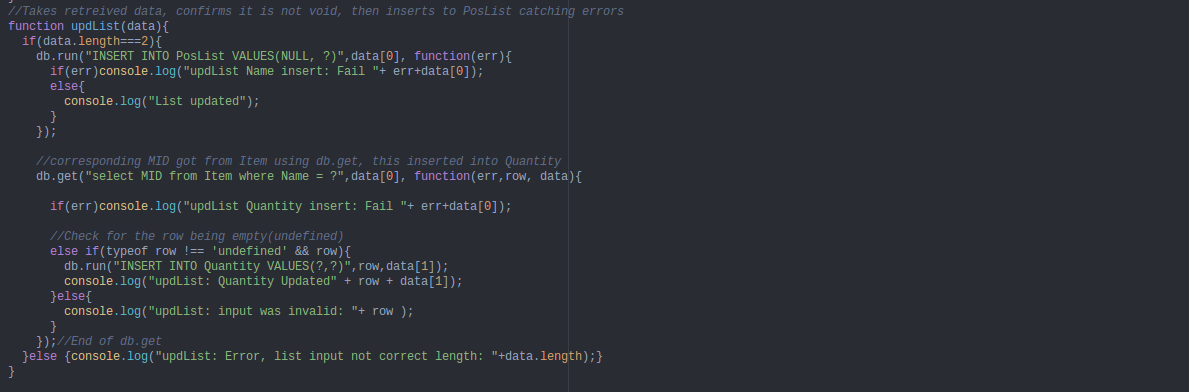
\includegraphics[width=\textwidth]{ProblemwithMID.png}
\label{foreignkey}
\caption{The stop statement returns the Key corresponding to the input item name. This is passed through the db.get callback to a second statement which inserts this value as well as the Quantity value in the Quantity table. The Name(in the data var) wasn't able to be accessed within the nested function however.}
\end{figure}

\subsection{Misc}
All text inputs were converted to lowercase. This was mainly to help when using them in other operations, such as checking for duplicates ect.. This could be changed to camel case, or this conversion done on a copy for aesthetic reasons. 


\bibliography{FridgeReport}
\bibliographystyle{plain}
\end{document}